\documentclass[11pt]{article}

\usepackage[margin=0.75in]{geometry}
\usepackage{url}
\usepackage{graphicx}
\usepackage{float}
\usepackage{amsmath}
\usepackage[utf8]{inputenc}
\PassOptionsToPackage{usenames,dvipsnames,svgnames}{xcolor}
\usepackage{tikz}
\usetikzlibrary{arrows,positioning,automata}
\graphicspath{ {../../graphs/} }
\usepackage{hyperref}
\usepackage{url}
\usepackage{listings}

%%% Date formatting to include month and year only
\usepackage{datetime}
\newdateformat{monthyeardate}{\monthname[\THEMONTH] \THEYEAR}

%%% Title
\title{A reproducible re-analysis of the RNA-seq study of
  \href{http://www.nature.com/neuro/journal/v18/n1/abs/nn.3898.html}{Jaffe
  \textit{et al.} (2014)}
}
%\subtitle{Reproducible Research in Bioninformatics and Statistics}

\author{ Nima Hejazi \\
  \href{mailto:nh@nimahejazi.org}{\texttt{nh@nimahejazi.org}}
}
\date{\monthyeardate\today}
\bibliographystyle{siam}

%%% Begin document
\begin{document}
\maketitle


\section{Introduction}
The present project concerns the re-analysis of transcriptomic data from the
study described in the paper
{\href{http://www.nature.com/neuro/journal/v18/n1/abs/nn.3898.html}
{``Developmental regulation of human cortex transcription and its clinical
relevance at base resolution''}}, Jaffe \textit{et al.}, \textit{Nature
Neuroscience}.


\section{Pseudo-alignment of RNA-seq reads}
In order to quantify RNA-Seq reads, alignment against a reference transcriptome
must be performed, a procedure which results in tables of read counts for use in
downstream statistical analysis. Here, we take advantage of
\textbf{pseudo-alignment}, a novel development in sequencing algorithms, to
probabilistically align reads. Below, we describe pseudo-alignment and the
results of its application to the Jaffe \textit{et al.} data. Pseudo-alignment
of reads was the primary pre-processing step necessary for re-analysis of the
data; for all scripts in the pre-processing pipeline, see the GitHub link:
\url{https://github.com/nhejazi/neurodevstat/tree/master/preprocess}.


\subsection{Summary of pseudo-alignment procedure}
Pseudo-alignment is a novel process for quantifying a set of samples of RNA-Seq
reads by performing partial matching against a reference transcriptome. The
novel pseudo-alignment process, implemented in the command line tool
\textbf{kallisto}, takes into account all of the information contained in a set
of reads while reducing the computational burden imposed by more traditional
alignment techniques. The \textbf{kallisto} tool provides results similar to
that produced by other alignment software (\textit{e.g.}, \textbf{bowtie}),
while taking only a fraction of the time. For a complete description of
pseudo-alignment, consult the paper
{\href{http://www.nature.com/nbt/journal/v34/n5/full/nbt.3519.html}
{``Near-optimal probabilistic RNA-seq quantification''}}, Bray \textit{et al.},
\textit{Nature Biotechnology}.


\subsection{Results of pseudo-alignment procedure}
The pseudo-alignment procedure was implemented on the Jaffe \textit{et al.} data
through the use of the \textbf{kallisto} command line tool. Using a publicly
available trascriptome assembled from the GRCh38 (hg19) \textit{Homo sapiens}
genome, sets of paired-end RNA-Seq reads for each of the 12 subjects involved in
the study were pseudo-aligned, resulting in count tables mapping each set of
reads to \textbf{173,259} transcriptomic objects. \textit{Please note that while
similar quantification tools (e.g., Cufflinks) produce estimates of mappings of
isoforms, kallisto provides estimates of transcript abundance}. Though this is
the first time that I have used \textbf{kallisto} for alignment and RNA-Seq
quantification, elementary searches for the ``run\textunderscore info.json''
output file (from other unrelated projects) seem to suggest that the produced
transcript abundances are normal for \textbf{kallisto}. Tables of counts are
produced for each set of paired-end RNA-Seq reads for each subject in a
tab-separated file format; these files are suitable for concatenation into a
single count table containing quantification results for all subjects, which can
be used as input to a set of statistical analysis scripts after appropriate data
cleaning.


\subsection{Sample code for pseudo-alignment with Kallisto}
The Kallisto software package was used to perform pseudo-alignment of paired-end
RNA-seq reads. After installation, Kallisto is available as a command-line tool.
In order to invoke the Kallisto pseudo-aligner on each pair of RNA-seq reads, a
wrapper script was written (in Python) to pass a call to invoke the
pseudo-aligner to the shell. The full wrapper script is available on GitHub at
\url{https://github.com/nhejazi/neurodevstat/blob/master/preprocess/04_pseudoAlign.py}.
\textbf{Excerpted code is displayed below:}

\begin{lstlisting}[language=Python]
  import os
  import sys
  import subprocess
  import numpy as np

  dir_data = os.path.abspath(os.getcwd() + "/data/" + str(data_dir))
  dir_fastq = dir_data + "/" + fastq_dir
  dir_out = dir_data + "/" + out_dir

  samples = [s[:10] for s in os.listdir(dir_fastq)]
  samples = list(np.unique(samples))

  for i in samples:
      pseudoalign = ("kallisto quant -i" + " " +
                     "./data/Homo_sapiens.GRCh38.rel79.idx -o" + " " +
                     str(dir_data) + "/" + str(out_dir) + "/" + str(i) + " " +
                     "-b 100" + " " + dir_fastq + "/" + str(i) + "_1.fastq.gz"
                     + " " + dir_fastq + "/" + str(i) + "_2.fastq.gz")
      subprocess.call(pseudoalign, shell = True)
\end{lstlisting}


\section{Gene-level summarization of transcripts}
The R package \textbf{tximport} was used to summarize the transcripts
quantified by the \textbf{Kallisto} pseudo-aligner at the level of known genes.
This step in the pre-processing pipeline is necessary in order to justify the
downstream use of popular software packages for statistical modeling. R scripts
for performing this stage of bioinformatical and statistical pre-processing are
available in the \textit{munge} subdirectory of the GitHub repository for this
project (see this link
\url{https://github.com/nhejazi/neurodevstat/tree/master/munge}).
\textbf{Excerpted code for gene-level summarization is displayed below:}

\begin{lstlisting}[language=R]
  # summarize data from transcript to genes for modeling and inference
  txdf <- transcripts(EnsDb.Hsapiens.v79, columns = c("tx_id", "gene_name"),
                      return.type = "DataFrame")
  tx2gene <- as.data.frame(txdf)
  txi <- tximport(filenames, type = "kallisto", tx2gene = tx2gene,
                  reader = read_tsv) #, countsFromAbundance = "scaledTPM")

  pseudocounts_genes <- as.data.frame(txi$counts)
  colnames(pseudocounts_genes) <- sapply(strsplit(filenames, split = "/"),
                                         function(x) x[9])
  pseudocounts_genes$geneID <- rownames(pseudocounts_genes)
\end{lstlisting}


\section{Statistical analysis at the level of genes}

\subsection{Pre-processing of (pseudo)counts with Limma "voom"}
In order to analyze differential expression after summarizing transcripts at the
gene level, the linear modeling method of the popular R package \textbf{limma}
was employed, including the "voom" transformation for analyzing RNA-seq digital
sequencing data in the form of counts (or, in this case pseudocounts). In order
to adequately use this transformation, we first filter out all genes for which
there were less than 10 mapped reads across subjects \textit{on average}. After
this filtering step, the "voom" transformation, including quality weights for
samples was performed.  Sample code and the produced plot are displayed below:

\begin{lstlisting}[language=R]
  v_simple <- voomWithQualityWeights(pseudocounts_filtered, design_simple,
                                     normalization = "scale", plot = TRUE)
\end{lstlisting}

\begin{figure}[H]
\centering
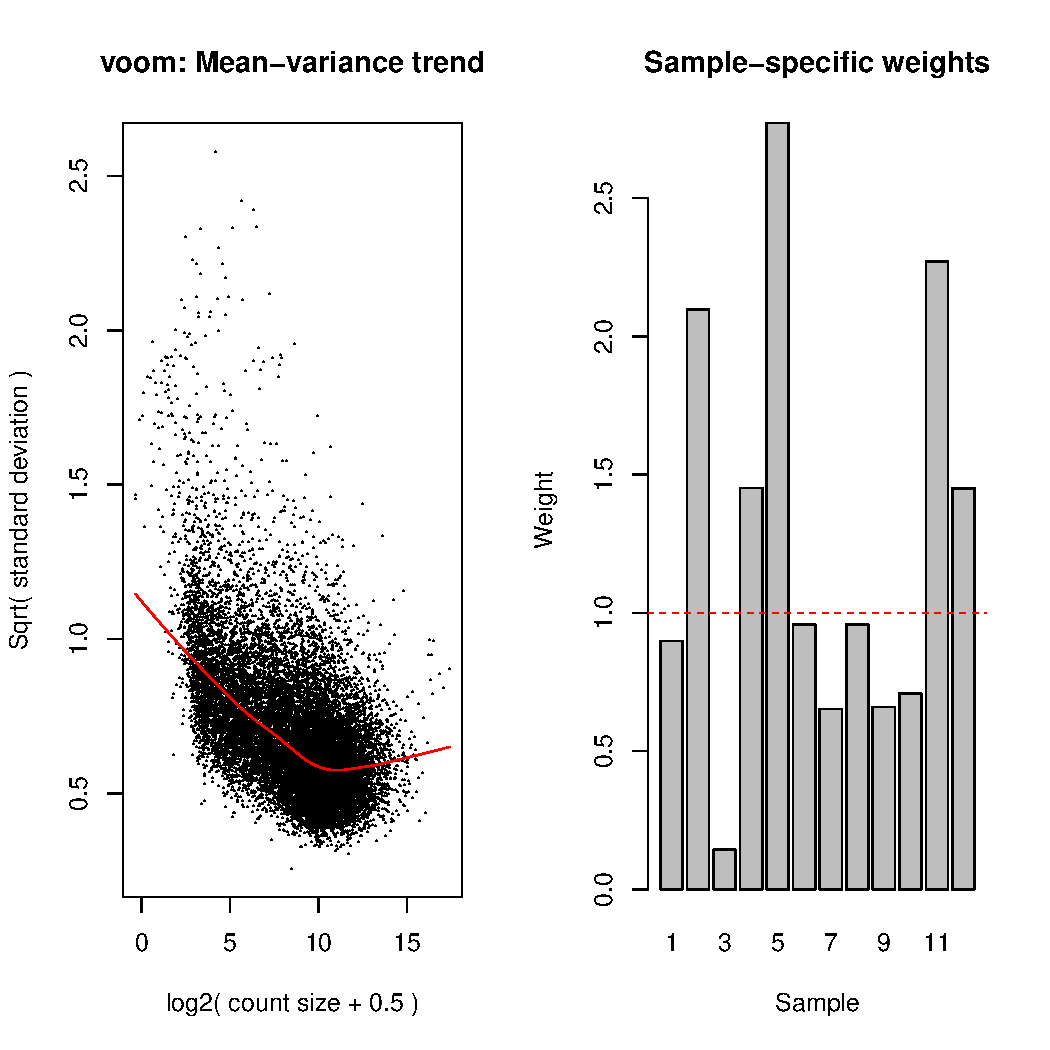
\includegraphics[scale=0.8]{voomTrend_simplemod.pdf}
\caption{Some description here.}
\end{figure}


\subsection{Statistical analysis via linear modeling with Limma}
Description here.

\begin{lstlisting}[language=R]
  vfit_simple <- limma::lmFit(v_simple)
  vfit_simple <- limma::eBayes(vfit_simple)
  tt1 <- limma::topTable(vfit_simple,
                         coef = which(colnames(design_simple) == "type"),
                         adjust.method = "BH", number = Inf,
                         sort.by = "none", confint = TRUE)
\end{lstlisting}

\begin{lstlisting}[language=R]
  aheatmap(exprs, scale = "row", annCol = label, annColors = "Set2",
           main = paste("Heatmap of Top", no_topgenes,
                        "Genes \n (ranked by FDR)"))
\end{lstlisting}

\begin{figure}[H]
\centering
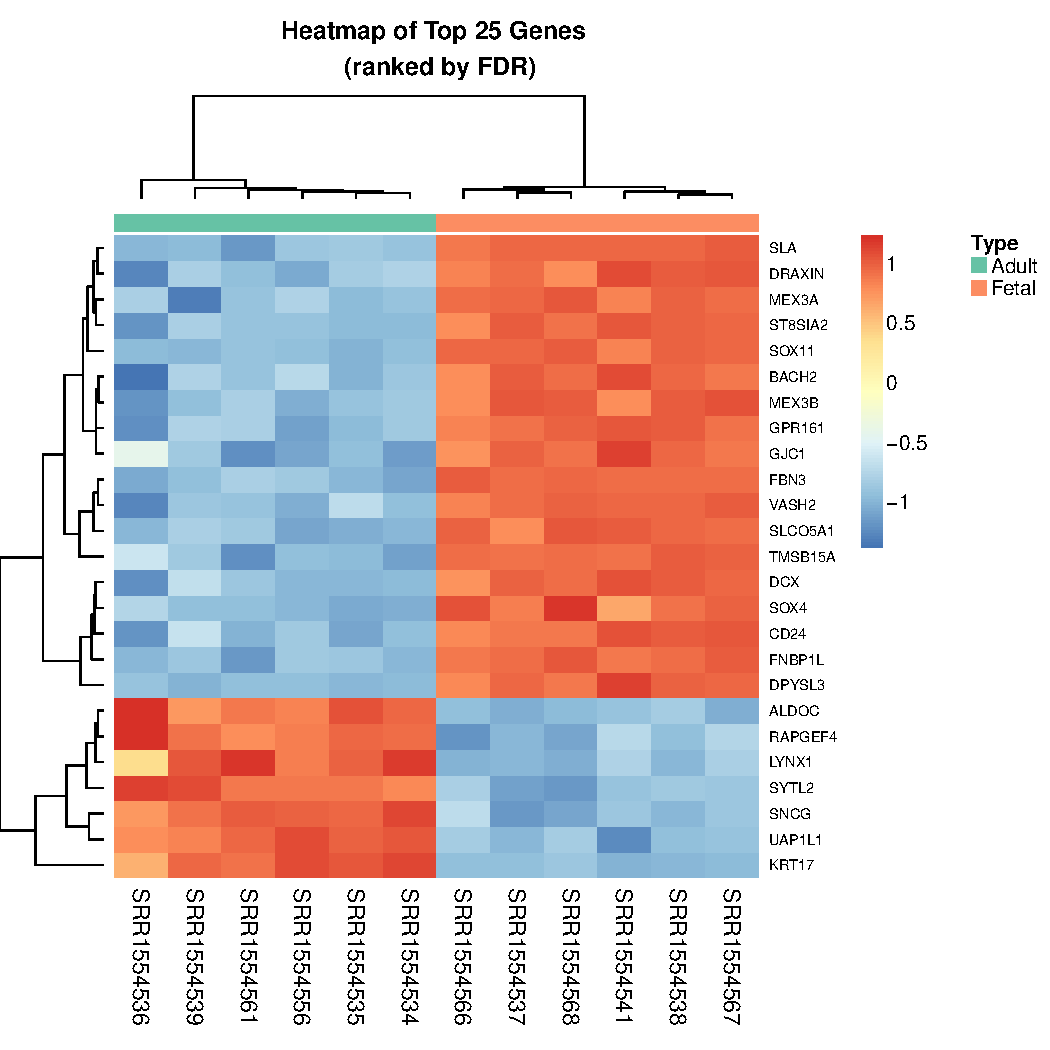
\includegraphics[scale=0.8]{heatmap_top25genes_simplemod.pdf}
\caption{Some description here.}
\end{figure}


\subsection{Results and Data Visualization}
Description here.

\begin{lstlisting}[language=R]
  p3 <- ggplot(tt_out1_gg, aes(x = logFC, y = logPval)) +
    geom_point(aes(colour = color)) +
    geom_text(aes(label = ifelse(top != 0, as.character(geneID), '')),
              hjust = 0, vjust = 0, check_overlap = TRUE) +
    xlab("log2(Fold Change)") + ylab("-log10(raw p-value)") +
    ggtitle("Volcano Plot \n (from simple model)") +
    scale_colour_manual(values = pal2[1:3], guide = FALSE)
  print(p3)
\end{lstlisting}

\begin{figure}[H]
\centering
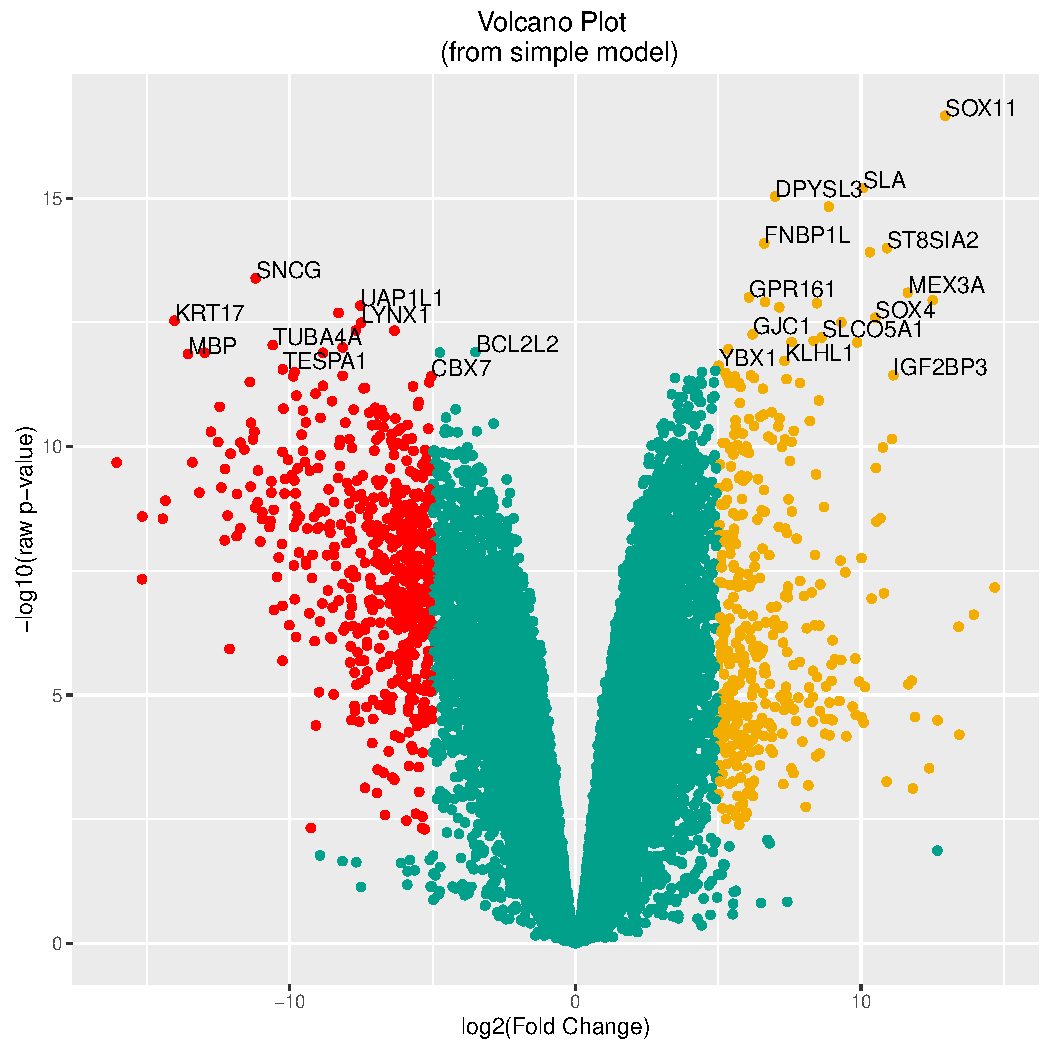
\includegraphics[scale=0.8]{volcano_simplemod_genes.pdf}
\caption{Some description here.}
\end{figure}


\section{Reproducibility notice}
In the spirit of computationally reproducible research, the material used
producing all of the analyses reported on in this project is publicly available
on GitHub at \url{https://github.com/nhejazi/neurodevstat}. Minimally sufficient
documentation is provided so that all reported results can be reproduced with
relative ease. With any concerns, contact the author at
\href{mailto:nh@nimahejazi.org}{nh@nimahejazi.org}.


\end{document}
